\section{Phase 1: Behebung grober API-Usability-Probleme}
\label{sec:phase1}

Die erste Einarbeitung in SeqAn und spätestens der erste \gls{gtm}-Analyseversuch der unter \ref{sec:programmierfortschritte} erläuterten \textit{Programmierfortschritte}-Datenquelle haben gezeigt, dass SeqAn teils offenkundige, schwere Usability-Probleme aufweist. Diese galt es in dieser ersten Phase zu beheben. Es bestand begründete die Befürchtung, dass derartige Probleme die Sicht auf die interessanten und tiefschürfenden API-Usability-Probleme verdecken. Insbesondere Dokumentationsprobleme, wie veraltete Installationsanleitungen, fehlende, kritische Dokumentationseinträge\footnote{U.a. waren die Konstruktoren der wohl wichtigsten Klasse --- nämlich der \texttt{String}-Klasse --- nicht dokumentiert.} und unzureichende Anwendungsbeispiele stellen starke Indizien für diese Befürchtung dar. Es ist davon auszugehen, dass derartige Lernhindernisse interessante Probleme gar nicht erst eintreten lassen. Es hat sich beispielsweise in der späteren Analyse gezeigt, dass manche Anwender bei zu großen Anfangsproblemen nicht weiter mit SeqAn arbeiten (siehe Seite \pageref{sec:gt-seqan-alternative}). Die genauen Ergebnisse dieser ersten Phase stelle ich weiter unten ab Seite \pageref{sec:phase1-ergebnisse} vor.

Um diese groben Probleme überhaupt systematisch aufzudecken, analysierte ich die Artefakte, auf die vermutlich ein Anwender trifft, wenn er das erste Mal SeqAn verwendet. Ich habe also die \textit{\gls{oobe}} \citep{Fouts:2000:SLE:353360.353375} von SeqAn mit Hilfe einer vereinfachten \textit{\glslink{he}{Heuristischen Evaluation (HE)}} analysiert.

Darüber hinaus habe ich während der ersten drei Datenerhebungsmöglichkeiten aus Triangulierungsgründen Befragungen unterschiedlicher Form durchgeführt (\textit{Workshop'11}: Online-Umfrage, \textit{PMSB'12}: Online-Umfrage und Interviews, \textit{Workshop'12}: Feedback-Zettel).

Die Datenanalyse diente, neben der Aufdeckung grober Usability-Probleme, auch der Verbesserung der SeqAn-Workshops selbst. Ein weiterer Nutzen war die Verbesserung meiner, für die Anwendung der \gls{gtm} notwendigen \textit{theoretischen Sensibilität}.



\subsection{Datenerhebung}

\subsubsection{\acrlong{oobe} relevante Artefakte}
\label{sec:oobe}

``Die \acrlong{oobe} --- kurz \acrshort{oobe} --- beschreibt die ersten Erfahrungen, die ein Anwender mit einem Produkt macht. Häufig hat der Anwender dabei --- abhängig von der Art des Produkts --- Kontakt mit den folgenden Artefakten: Produktverpackung und -handbuch, Installationsprozedur, Konfigurationsassistent, usw. \citep{Fouts:2000:SLE:353360.353375}''. \citep{Kahlert:2011wr}

Für die relevanten OOBE-Artefakte von SeqAn habe ich die Installationsanweisungen (\textit{Getting Started}), die drei Anfänger-Tutorials (\textit{Basics}, \textit{Sequences}, \textit{Iterators}) und die den SeqAn-Entwurf erklärenden Tutorials (insb. \textit{Metafunctions} und \textit{Template Subclassing}) betrachtet.

\subsubsection{Online-Umfrage}

Die Online-Umfrage hatte folgende Ziele:
\begin{description}
  \item[Vorerfahrung] Die Anwenderschaft von SeqAn sollte besser verstanden werden. Interessant waren allgemeine Programmiervorkenntnisse und spezielle Programmierkenntnisse in Bezug auf die in SeqAn eingesetzten Techniken (siehe \sref{sec:seqan-entwurf}).
  \item[Installation] Probleme bei der Installation eines Produkts sind inhärenter Bestandteil der OOBE und entsprechend auch für SeqAn von hoher Relevanz.
  \item[Tutorials] Auch die Tutorials sind wichtige OOBE-relevante Artefakte. Schließlich handelt es sich bei den Tutorials um \textit{die} Lernressource für SeqAn-Anfänger.
  \item[Bewertung] Persönliche Einschätzungen von SeqAn und dessen Gebrauch waren ebenfalls von Interesse für mich.  
\end{description}

Der vollständige Fragebogen befindet sich im \aref{app:umfrage}. Er enthält auch Fragen zur Organisation des SeqAn-Workshops, die aber nicht Gegenstand dieser Arbeit sind.

Der Fragebogen wurde unter Berücksichtigung von \cite{mayring2002einfhrung} entwickelt und mit Hilfe von \textit{LimeSurvey}\footnote{\url{https://www.limesurvey.org}} implementiert und bereitgestellt.

Die Online-Umfrage wurden im Anschluss an den praktischen Teil des Workshops'11 und nach der SeqAn-Einführung des PMSB'12-Praktikums eingesetzt.

Insgesamt nahmen 18 Teilnehmer an der Umfrage teil.


\subsubsection{Interviews}

Neben der Online-Umfrage habe ich während des PMSB'12-Praktikums mit vier Teilnehmern jeweils ein offenes Interview \citep{mayring2002einfhrung} geführt. Dabei interessierten mich Probleme, auf die die Studenten beim Gebrauch von SeqAn stießen.


\subsubsection{Feedback}
\label{sec:feedback}

Bei der Durchführung der Online-Umfrage musste ich feststellen, dass eine nicht kleine Anzahl Workshop-Teilnehmer sich nicht an der Online-Umfrage beteiligte, was auf Teilnehmerseite nachvollziehbar, aber für meine Forschung nachteilig war.

Basierend auf den Erfahrungen der beiden Online-Befragungen habe ich einen Feedback-Zettel erstellt, der um weitere Fragen ergänzt wurde. Die neuen Fragen (u.a. Motivation für Bearbeitung eines Tutorials; Anwendungsform von SeqAn) bezweckten ein besseres Verständnis der SeqAn-Anwendergruppe.

Des Weiteren habe ich den Befragungsmodus geändert. Statt eine Befragung am Ende des gesamten dreitägigen Workshops durchzuführen, sollte je ein Fragebogen am Anfang der des Workshops, im Anschluss an jedes Tutorial und am Ende des Workshops ausgefüllt werden.

Die drei Feedback-Fragebogen-Varianten (Einstieg, Tutorial, Abschluss) befinden sich vollständig im \aref{app:feedback}.

Insgesamt wurden 210 Feedback-Zettel von max. 58 Entitäten ausgefüllt. Die genaue Anzahl der Beteiligten kann nicht bestimmt werden, da nicht jeder Teilnehmer seine Feedback-Zettel mit einem selbst gewählten Pseudonym markiert hat (Details siehe \sref{sec:id}). Dadurch konnten die verschiedenen Feedback-Zettel nicht einer Person zugeordnet werden und mussten separat analysiert werden.


      
\subsection{Datenanalyse}
\label{sec:he}

Für die Analyse der eben beschriebenen Daten habe ich, neben einfachen quantitativen Mitteln (vgl. \sref{sec:schwierigkeiten}), die \acrfull{he} eingesetzt.

Die \gls{he} wurde erstmalig von \cite{Nielsen:1990bw} und praxisbezogener von \cite{Nielsen:1994tx,Nielsen:1993vk} beschrieben. Sie wird dem \textit{Discount-Usability-Engineering} zugesprochen \citep{Sarodnick:2006vc}; stellt also ein kostengünstiges Verfahren zur Usability-Evaluation dar. Das Verfahren sieht vor, dass Usability-Experten Artefakte eines Softwaresystem mit der Perspektive des Anwenders gedanklich verarbeiten und dabei Verstöße gegen die vorher definierten Heuristiken aufdecken. Heuristiken haben ihren Namen von der Tatsache, dass ein Verstoß nur auf ein Usability-Problem hindeutet, es jedoch nicht beweist und die Heuristiken auch nicht alle existierenden Probleme aufdecken.

Dem ursprünglichen Verfahren liegen zehn Heuristiken zu Grunde, die ich im \aref{app:heuristiken} aufführe. 

Beim Versuch, die originären Heuristiken anzuwenden, stellte ich fest, dass sie sich nicht für die Evaluation meiner Artefakte eignen. Das betrifft insbesondere die Heuristiken \textit{Sichtbarmachung des Systemstatus}, \textit{Benutzerkontrolle und -freiheit}, \textit{Wiedererkennen, statt sich erinnern}, \textit{Flexibilität und Effizienz der Benutzung} und \textit{Ästhetik und minimalistisches Design}. Der Grund: Diese Heuristiken haben einen starken Bezug auf grafische Benutzeroberflächen, die es im Falle von SeqAn nicht gibt. Natürlich kann man Elemente von APIs beispielsweise unter ästhetischen Gesichtspunkten betrachten. Dass eine geringe Ästhetik jedoch ein hinreichend sicher auf ein Usability-Problem hindeutet, ist nicht empirisch gezeigt und stellt damit auch keine praktikable Heuristik dar.   

An dieser Stelle stand ich also vor der Wahl, speziell für die Evaluation von APIs geeignete Heuristiken herzuleiten oder lediglich die verbliebenen Heuristiken zu verwenden und mich auf meine \gls{he}-Anwendungserfahrung  \citep[vgl.][]{Kahlert:2011wr} zu verlassen. Ich habe mich für die zweite Variante aus den folgenden Gründen entschieden:

\begin{enumerate}
  \item Die theoretische bzw. literaturbasierte Herleitung von Heuristiken entspricht nicht meiner Vorstellung von explorativer Forschung. Ich befürchtete, dass eine zu intensive Auseinandersetzung mit API-relevanten Heuristiken meine \gls{gtm}-Forschung --- insbesondere beim offenen Kodieren --- verzerren und die in den Daten verankerte Theorie nicht mehr korrekt wiedergeben würde.
  \item Für einen speziellen Untersuchungsgegenstand individuelle Heuristiken zu entwickeln, ist nicht trivial \citep{Nielsen:1993vk}. Die von \cite{Grill:2012jm} entwickelten API-Heuristiken wurden erst nach meiner Analyse veröffentlicht. Allerdings sehe ich das Zustandekommen dieser Heuristiken kritisch (siehe \sref{sec:grill-kritik}.
  \item Die Bereinigung der groben Usability-Probleme stellte ``nur'' ein notwendiges und vor allem unvorhergesehenes Übel dar. Da ich mich mit der \gls{he} gut auskenne und es nicht um die Kategorisierung, sondern um die Beseitigung von Problemen ging, habe ich mir die mühsame Problem-Klassifikation erspart.
\end{enumerate}




\subsection{Ergebnisse}
\label{sec:phase1-ergebnisse}

Die Ergebnisse meiner \gls{he} sind vollständig im \aref{app:he-ergebnisse} beschrieben. Insgesamt habe ich 59 Usability-Probleme gefunden, von den 32 schwer oder katastrophal\footnote{\cite{Nielsen:1994tx} formulieren die folgenden Fatalitäten:\\0 = \textit{Kein Usability-Problem}, 1 = \textit{Kosmetisch}, 2 = \textit{Gering}, 3 = \textit{Schwer}, 4 = \textit{Katastrophal}.} waren. Im Folgenden beschränke ich mich auf die Darstellung der wichtigsten Ergebnisse.

Die Auswertung habe ich ursprünglich in \textit{Apple Numbers} vorgenommen (siehe \fref{fig:analysis-keynote}) und später auf \textit{Wolfram Mathematica} umgestellt.
%TODO: Screenshot von Datei auf rugi.imp.fu-berlin.de

\begin{figure}
  \centering
    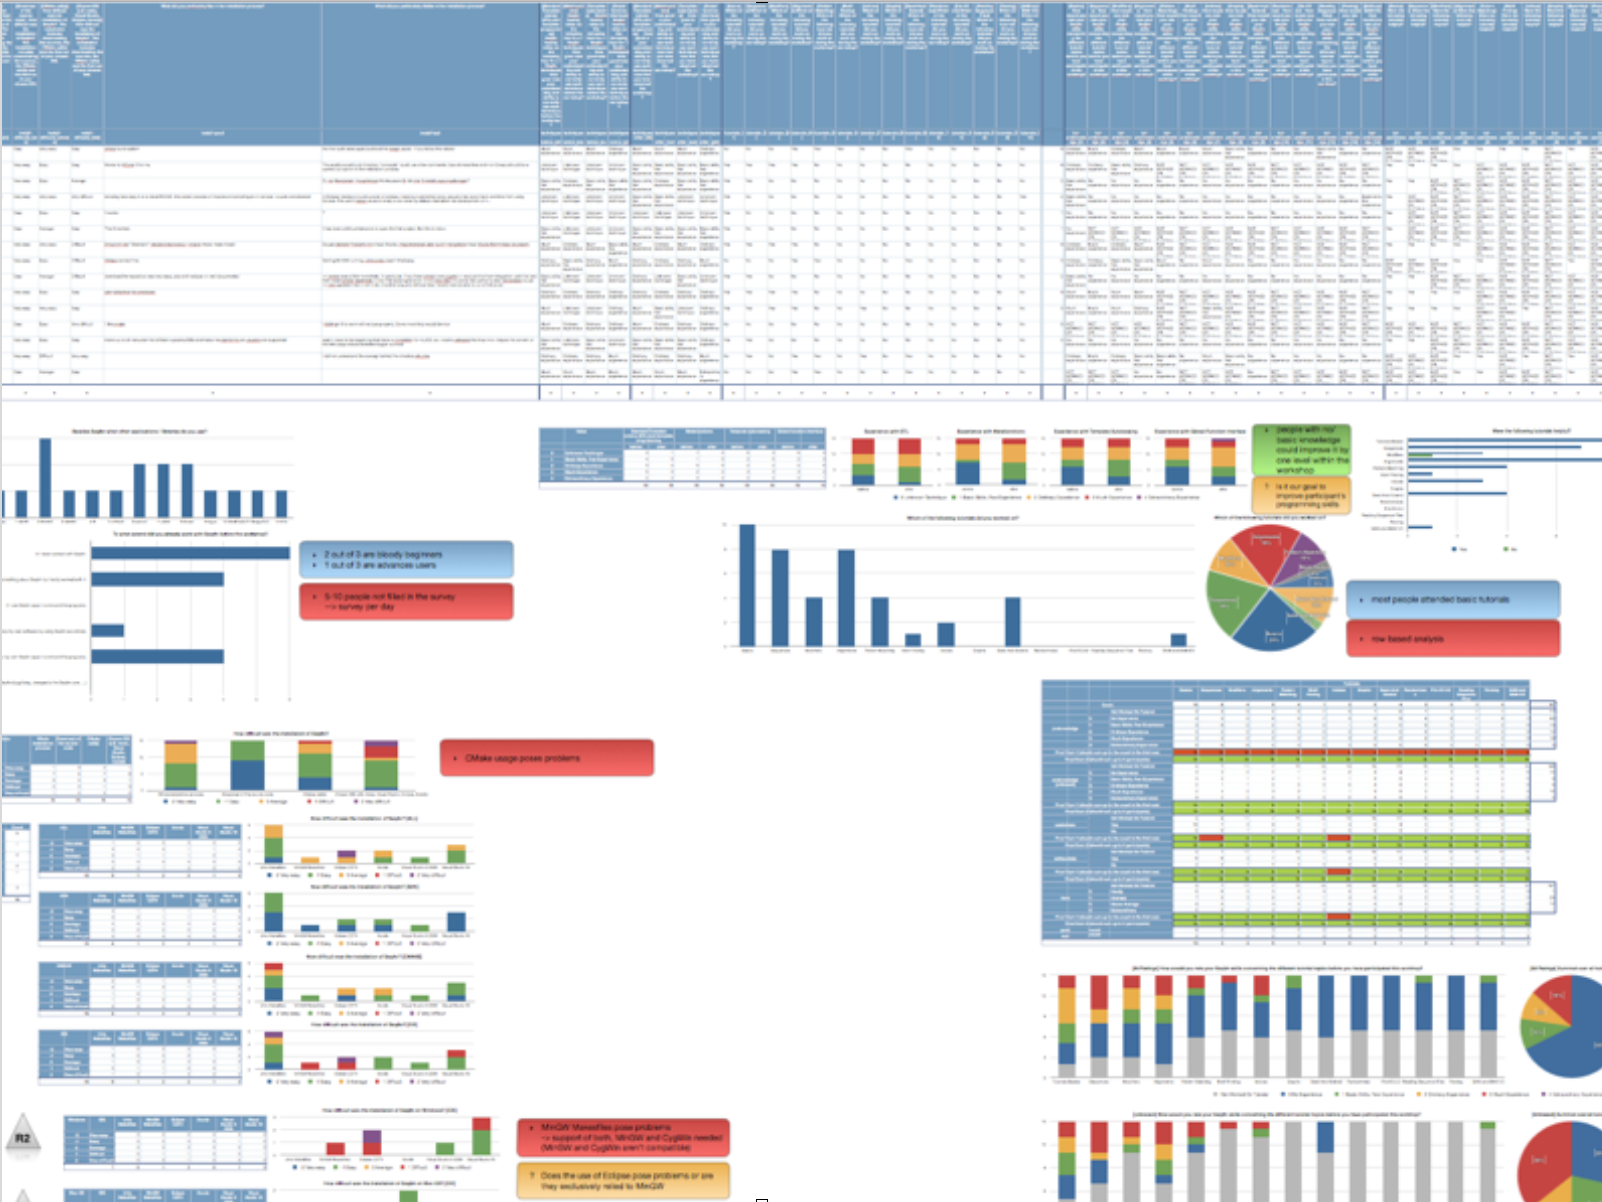
\includegraphics[width=0.75\linewidth]{Figures/analysis-keynote.png}
  \caption{Erste Analyse in Apple Keynote}
  \label{fig:analysis-keynote}
\end{figure}


\subsubsection{Anwender}
\label{sec:results-users}

Die Anwendergruppen habe ich qualitativ und quantitativ analysiert. Die Anzahl der betrachteten Anwender beträgt 35. Wegen diese geringe Anzahl, dem Workshop-Format und der subjektiven Einschätzung der Anwender selbst, kann man nicht davon ausgehen, dass die Ergebnisse verallgemeinerbar sind. Dennoch geben sie einen plausiblen Anhaltspunkt für die Charakterisierung der Anwenderschaft.

\begin{itemize}
  \item In gleichen Teilen waren Studenten und berufstätige Wissenschaftler vertreten.
  \item Jeweils knapp die Hälfte der Teilnehmer kam aus der Bioinformatik und Informatik. Aus der Biotechnologie, der Molekularbiologie und der Physik kamen jeweils einer der 35 Teilnehmer.
  \item Häufig wurden ``Effizienz'', ``Geschwindigkeit'' und ``Performance'' als Motivation zur Auseinandersetzung mit SeqAn formuliert.
  \item Etwa die Hälfte der Anwender nutzt \textit{Microsoft Windows}, ein Drittel \textit{Linux} und die übrigen \textit{Mac OS X}.
  \item Die Hälfte der Anwender nutzte eine integrierte Entwicklungsumgebung. Die andere Hälfte nutzte Makefiles.
  \item Mehr als zwei Drittel der Teilnehmer verfügt über fortgeschrittene Kenntnisse im Gebrauch von objektorientierter Programmierung in den Sprachen C{}\verb!++! oder Java.
  \item C{}\verb!++!-Kenntnisse sind gleich verteilt (jeweils ein Drittel Anfänger, Fortgeschrittene und Experten).
  \item Erfahrungen in Bezug auf den von SeqAn eingesetzten Techniken waren wenig vorhanden (Beispiel \textit{Metafunktionen}: nur 20\% fortgeschrittene Kenntnisse oder besser).
  \item Einige Anwender gaben an, dass sie von der SeqAn-Installation abgeschreckt waren. Hätten sie nicht am Workshop teilgenommen, hätten sie die Installation abgebrochen und sich nach einer anderen API umgesehen. Diese Beobachtungen machten auch \cite{sunshine2014searching}.
\end{itemize}



\subsubsection{Dokumentation}

\begin{itemize}
  \item 2 von 3 Befragten hielten die Dokumentation für mangelhaft beschrieben (vgl. \fref{fig:dox-index-old}).
  \item Den Befragten fehlten vor allem eine Einführung, Beispiele und Verlinkungen zu den Tutorials.
  \item Eine Begründung und Motivation für die Entscheidung, Templatemetaprogrammierung einzusetzen, fehlt.
  \item Es fehlen Best-Practise-Beschreibungen (z.B. \texttt{++var} oder \texttt{var++}?).
  \item Es fehlt die Beschreibung von Benennungsregeln/-konventionen für Variablen, Funktionen, etc.
\end{itemize}

\begin{figure}
  \centering
    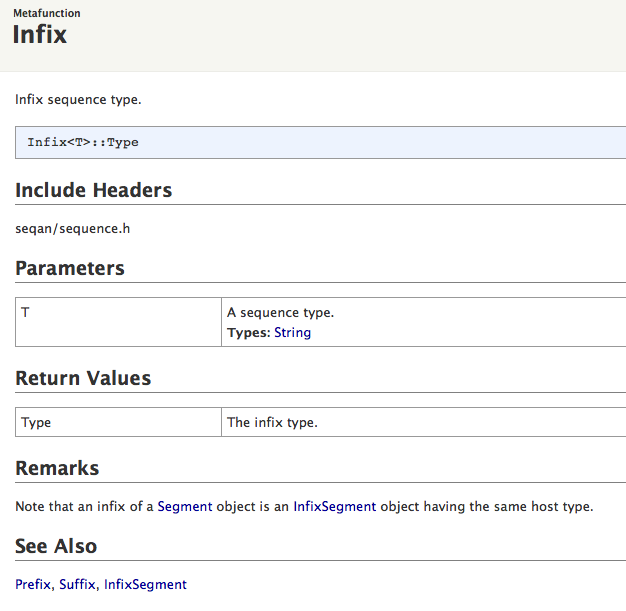
\includegraphics[width=0.95\linewidth]{Figures/dox/infix-old.png}
  \caption[Mangelhafter Dokumentationseintrag]{Mangelhafter Dokumentationseintrag zur Metafunktion \texttt{Infix},\\Stand: 02.07.2012}
  \label{fig:dox-index-old}
\end{figure}


\subsubsection{Tutorials}

\begin{itemize}
  \item Die Tutorials haben einen zu hohen Anspruch.
  \item Die Tutorials sind von geringer didaktischer Qualität.
  \item Die Tutorials verfügen über keinerlei explizite Meta-Angaben wie Zielgruppe, Schwierigkeitsgrad, etc.
  \item Die Qualität der Tutorials variiert eklatant.
\end{itemize}



\subsubsection{Installation}

\begin{itemize}
  \item Die Installation wurde mehrheitlich als schwierig beschrieben.
  \item Hauptgrund 1: Mängel in der Installationsanleitung (inkonsistent, fehlerhaft)
  \item Hauptgrund 2: SeqAn hat sich als Framework und nicht als Softwarebibliothek entpuppt. Dieser Punkt wird ausführlicher im \sref{sec:library-vs-framework} erläutert.
\end{itemize}



\subsubsection{Softwarebibliothek}

\begin{itemize}
  \item Den Anwendern war nicht klar, weshalb SeqAn die ``komplizierte'' Templatemetaprogrammierung verwendet. Die Mehrheit der Teilnehmer erwartete, dass SeqAn auf Objektorientierung basiert. Ein Teilnehmer bezeichnete SeqAn sogar als ``Vergewaltigung der OO-Programmierung''\citepurl{apiua://survey/2011-09-14-T15:23:17.211+02:00}. Dieser Punkt hat sich als äußerst relevant herausgestellt und wird u.a. im \sref{sec:lie-oop} besprochen.
  \item Die \mintinline{cpp}{length}-Funktion gibt alle Eingaben, für die sie nicht explizit entwickelt wurde, \texttt{1} zurück.
  \item Es wurden mehrere funktionale Schwächen gefunden. Beispiel: Die Konkatenierung eines SeqAn-Strings und eines C{}\verb!++!-Strings war nicht mit dem \texttt{+}-Operator möglich.
  \item Funktionen sind nur schwer aufzufinden, denn sie gehören keiner Klasse an.
  \item Mehrfach wurde das Fehlen der \texttt{substring}-Funktion zur Erzeugung von Teilstrings, bemängelt.
\end{itemize}

All die hier genannten Punkte sind von großer Relevanz, wie die spätere \gls{gtm}-Analyse gezeigt hat.



\subsubsection{Zusammenfassung der Ergebnisse}

Mit meiner Analyse der OOBE-Artefakte und den, in zwei SeqAn-Workshops und einem PMSB-Praktikum erhobenen Daten konnte ich zu einer besseren Charakterisierung der SeqAn-Anwendergruppe beitragen und teilweise schwerwiegende Probleme in der Dokumentation, den Tutorials, sowie bei der Einrichtung und bei dem Gebrauch von SeqAn aufdecken.

Als größtes Usability-Problem hat sich die Erlernbarkeit von SeqAn herausgestellt. Es gibt Indizien dafür, dass diese Anwender von der Verwendung von SeqAn abschrecken. Das Usability-Problem hat zwei Ursachen:
\begin{enumerate}
  \item Die Dokumentation ist von vergleichsweise geringer Qualität, die bei den verschiedenen Dokumentationseinträgen variiert.
  \item SeqAn setzt auf das Programmierparadigma Templatemetaprogrammierung. Dies stellt Anwender mit C{}\verb!++!-Vorerfahrung vor das Problem, dass dieser Ansatz sich stark von der C{}\verb!++! Standard (Template) Library unterscheidet. Anwender mit Java-Vorerfahrung vermissen die Ähnlichkeit zur objektorientierten Softwareentwicklung.
\end{enumerate}

Das Problem der Erlernbarkeit spielt eine wichtige Rolle im späteren Teil dieser Arbeit. Die Behebung vieler anderer Probleme wird im folgenden Abschnitt vorgestellt.





\subsection{Verbesserungen}

Jedes Usability-Problem isoliert zu lösen, ist aus praktischer Sicht weder möglich noch effizient. Viel mehr Sinn macht es, Maßnahmen zu formulieren, die eine ganze Gruppe von Usability-Problemen beheben.

Für die Behebung der gefundenen Usability-Probleme, habe ich Maßnahmen definiert und eine Maßnahmen-Probleme-Zuordnung vorgenommen. Den Aufwand einer jeden Maßnahme habe ich in Stunden geschätzt. Der Nutzen einer Maßnahme wiederum, ergibt sich aus der Anzahl und der \textit{Fatalität} der durch sie behobenen Usability-Probleme.

Zu den wichtigsten formulierten Maßnahmen gehören:
\begin{itemize}
\itemsep1pt\parskip0pt\parsep0pt
  \item Vollständige Überarbeitung und Vereinheitlichung der Installationsanleitungen
  \item Definition von Anforderungen für Tutorials
  \item Bereitstellung einer Vorlage für Tutorials
  \item Anpassung sämtlicher Tutorials an Anforderungen und Vorlage
  \item Erstellung eines neuen Anfänger-Tutorials
  \item Einführung von Aliassen in der Dokumentation (Auffindbarkeit von Einträgen durch Synonyme)
\end{itemize}

Die vollständige Zuordnung, samt der Kosten-/Nutzen-Schätzungen, befindet sich im \aref{app:he-massnahmen}. Es wurden vornehmlich die Arbeitspakete umgesetzt, die nicht die Softwarebibliothek im engeren Sinne selbst betreffen. Für die Verbesserung der Softwarebibliothek selbst sollte die, im \sref{sec:phase4} beschriebene Phase 4 dienen.

\bigskip

Im Folgenden stelle ich die tatsächlichen Änderungen vor. Meine organisatorischen und inhaltlichen Verbesserungen der SeqAn-Workshops sind nicht Gegenstand dieser Arbeit und werden daher nicht vorgestellt. 


\subsubsection{Prozessverbesserungen}

\paragraph{Commit-Nachrichten}

Die SeqAn-API-Entwickler haben ihre Commit-Nachrichten für ihr Versionsverwaltungssystem nach Belieben formuliert. Diese erschwerte die Nachvollziehbarkeit von Code-Änderungen für die Entwicklerkollegen. Für mich war dieses Format ebenso wichtig, da ich für meine Analyse darauf angewiesen war, wichtige Änderungen des SeqAn-Codes zu erfahren (vgl. \sref{sec:schwierigkeiten}). Allein für den Versionssprung von SeqAn 1.3 auf 1.4 gab es rund 3.500 Commits.

Zu Vereinheitlichung haben mein Kollege Manuel Holtgrewe und ich ein Format entwickelt, das ausführlich online\footnote{\url{http://seqan.readthedocs.org/en/master/HowTo/WriteCommitMessages.html}} beschrieben wird. Darüber hinaus habe ich einen positiv angenommenen ``Spickzettel'' (siehe \fref{fig:commit-messages-format}) erarbeitet, auf den API-Entwickler zurückgreifen können.

\begin{figure}
  \centering
    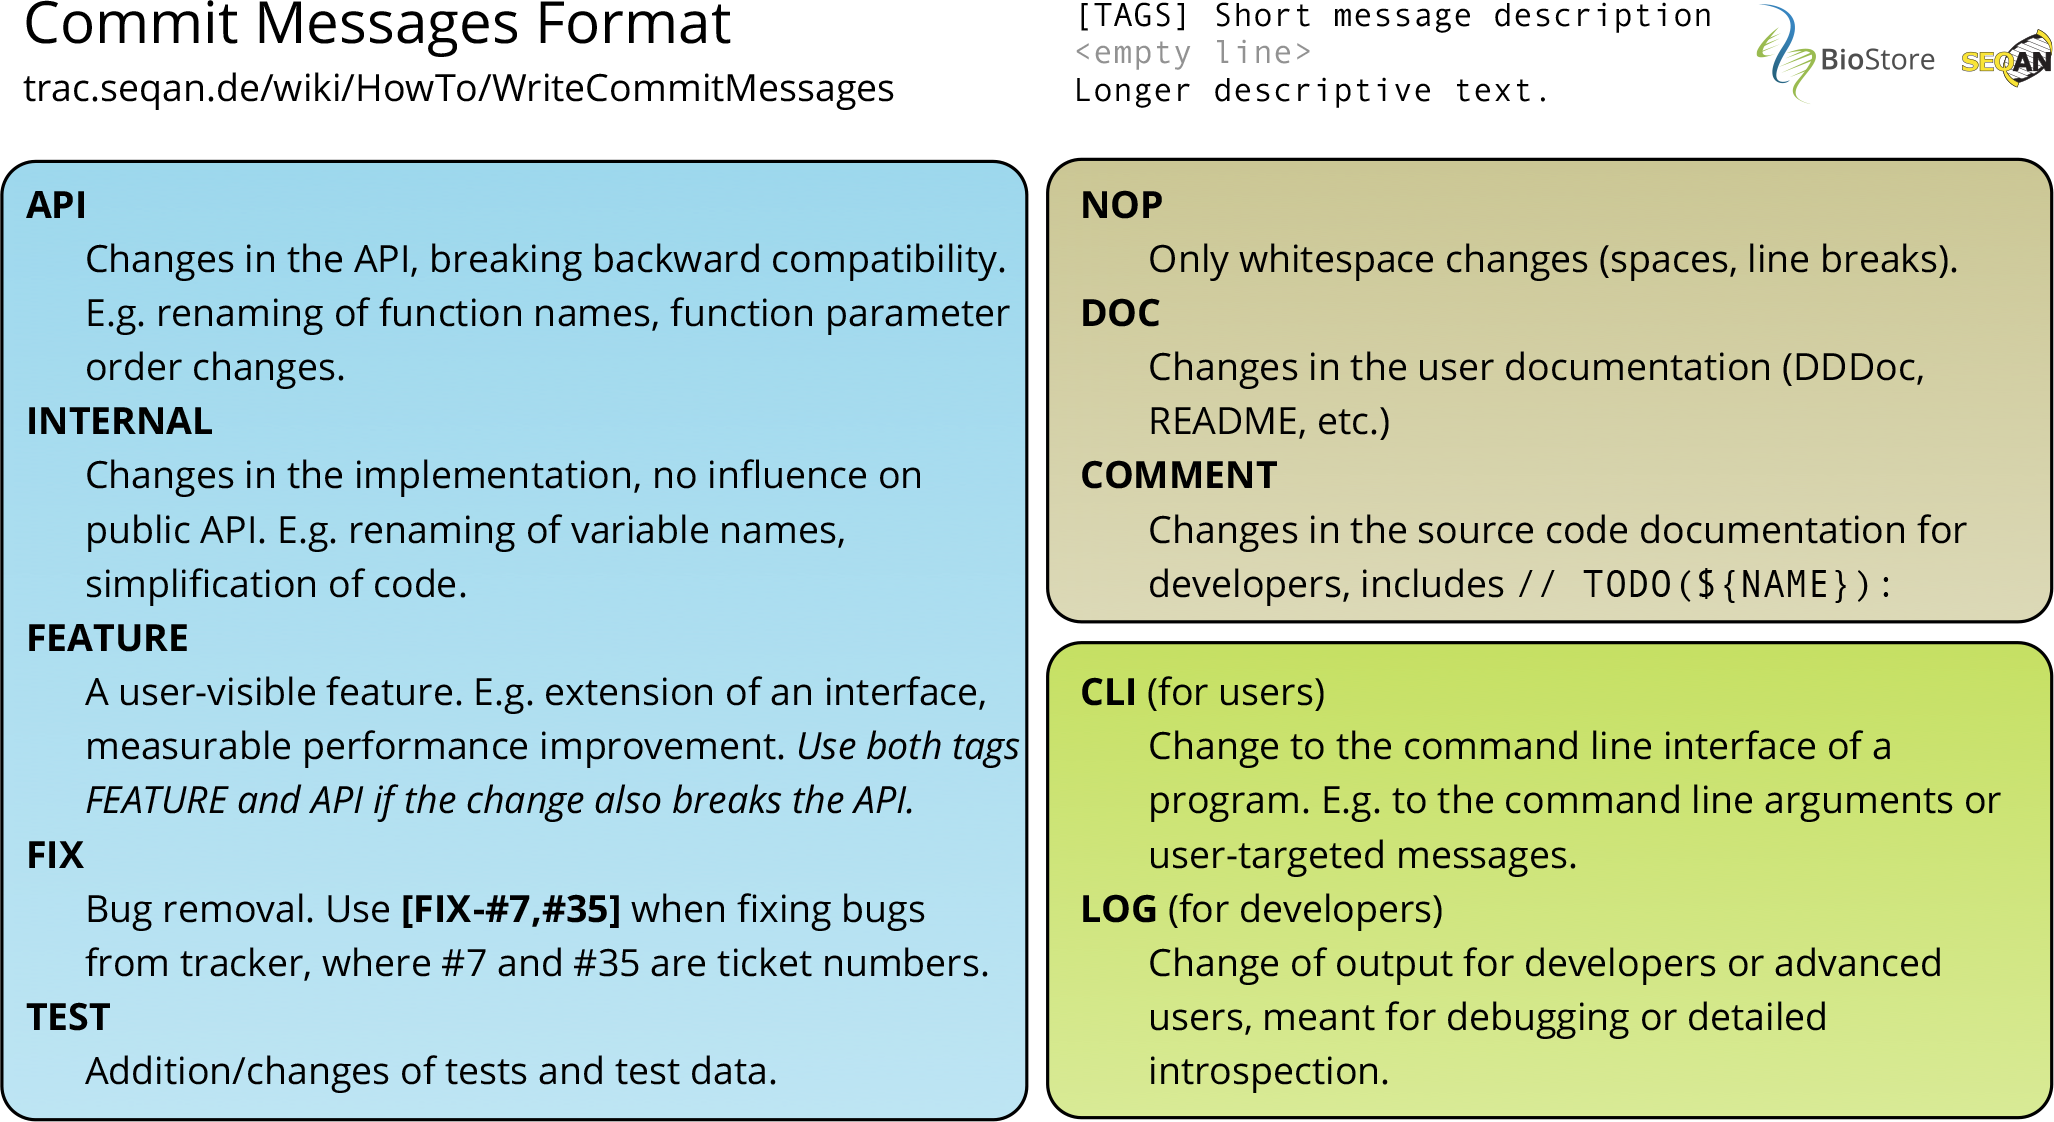
\includegraphics[width=0.9\linewidth]{Figures/20120504-CommitMessagesFormat.png}
  \caption[Commit-Nachrichten-Format]{Standardisiertes Format für Commit-Nachrichten}
  \label{fig:commit-messages-format}
\end{figure}


\paragraph{Umstellung Subversion auf Git}

In der Bioinformatik-Arbeitsgruppe arbeiten viele Mitarbeiter an einer einzigen SeqAn-Anwendung im Rahmen ihrer Tätigkeit. Dies führte durch den Gebrauch des zentralen Versionsverwaltungssystems \textit{Subversion} dazu, dass SeqAn nach dem Commit von Codeänderungen nicht mehr kompilierte.

Um SeqAn-Entwicklern eine größere Freiheit und Sicherheit zu geben, indem sie Änderungen lokal revisionieren können, wurde eine Umstellung auf \textit{Git} vorgenommen. Im Zuge dieser Umstellung wurden die Kollegen geschult und ein SeqAn-Git-Workflow\footnote{\url{http://seqan.readthedocs.org/en/master/Infrastructure/SeqAnWorkflow.html}} basierend auf dem prominenten Gitflow\footnote{\url{https://www.atlassian.com/git/tutorials/comparing-workflows/gitflow-workflow}} formuliert und etabliert.



\paragraph{Code-Reviews}

Die Entwicklung von SeqAn-Code unterlag keiner praktischen Qualitätssicherung. Aus diesem Grund habe ich angeregt, Codeinspektionen (\textit{Code-Reviews}) durchzuführen.

Diese Qualitätssicherungsmaßnahme wurde schließlich in den Commit-Prozess als Prä-Commit-Review integriert. Durch die spürbare Verlangsamung des Entwicklungsprozesses, haben die SeqAn-Entwickler, im Zuge der Git-Umstellung, auf das Post-Commit-Review gewechselt. Das heißt, Commits werden nun erst inspiziert, wenn sie bereits in den Code integriert wurden. Für externe Entwickler gilt weiterhin ein Prä-Commit-Verfahren, das durch die Arbeitsweise von Git leicht zu implementieren war.




\subsubsection{Argument-Parser}
\label{sec:argument-parser}
Für die sich vornehmlich an Wissenschaftler richtende Workflow-Engine KNIME wurde basierend auf einer Vorarbeit der Universität Tübingen\footnote{\url{http://www.knime.org/files/ugm2013_talks/knime_ugm_2013_knutreinert_final.pdf}} ein generischer Wrapper für Konsolenanwendungen zur Bereitstellung von SeqAn-Awendungen in KNIME entwickelt\footnote{\url{https://github.com/genericworkflownodes}}.

Dieser, unter dem Namen \textit{GenericWorkflowNodes} firmierende Wrapper nutzt ein XML-basiertes Datenformat zur Beschreibung seiner Ein- und Ausgabeschnittstelle. Konsolenanwendungen verfügen selbst bereits auch schon über eine beschriebene Schnittstelle, auch wenn diese nur --- möglicherweise über das ganze Programm verstreut --- programmatisch beschrieben ist.

Um eine redundante Schnittstellenbeschreibung --- nämlich einmal im Programm und einmal in der KNIME-Knotenbeschreibung --- zu vermeiden, wurde eine neue Komponente zum Parsen von Argumenten geschrieben. Diese kann sowohl die Hilfebeschreibung einer Konsolenanwendung mittels des Parameters \texttt{--help} bzw. \texttt{-h}, eine Manpage, eine HTML-Dokumentation, als auch eine  KNIME-Knotenbeschreibunsdatei ausgeben.

Dieser Argument-Parser wurde in der ersten Version von mir und später von meinem Kollegen Stephan Aiche weiterentwickelt und perfektioniert. Der Parser unterstützt ein breites Spektrum an Funktionen, das von zahlreichen Parametertypen (\textit{flag options}, \textit{value options}, \textit{positional options}, \ldots) bis hin zu Restriktionen (Typisierung, Wertebereiche, Datentypen, \ldots) reicht.

Sämtliche SeqAn-Anwendungen wurden an den neuen Argument-Parser angepasst. Dessen Verwendung stellt eine API-Usability-Verbesserung sowohl für API-Entwickler als auch für API-Anwender dar.

\bigskip

\begin{samepage}
API-Entwickler profitieren von einer einfachen, mächtigen Komponente zur Beschreibung der Schnittstelle (siehe \lref{lst:argparser-interface}) und dem Beziehen von Parametern.

\begin{center}
\begin{minted}[linenos, firstnumber=1]{cpp}
seqan::ArgumentParser parser("Argument-Parser Demo");

setShortDescription(parser, "Basic functionality of the Argument-Parser");
setVersion(parser, "0.1");
setDate(parser, "2013-09-18");

addUsageLine(parser, "[OPTIONS] \"TEXT\"");
addDescription(parser, "This program allows simple string repetition by i times.");

addSection(parser, "Demo Options");
addOption(parser, seqan::ArgParseOption("i", "times", "Number of repetitions.", seqan::ArgParseArgument::INTEGER, "INT"));

setDefaultValue(parser, "times", 1);
addTextSection(parser, "Examples");
addListItem(parser, "modify_string -i 5 \"text\"", "Print \"text\" 5 times");
\end{minted}
\captionof{listing}{Argument-Parser: Beispielhafte Schnittstellenbeschreibung in C\texttt{++}}
\label{lst:argparser-interface}
\end{center}
\end{samepage}

\bigskip

\begin{minipage}{\textwidth}
API-Anwendern stehen nun einheitlich und ausführlich beschriebene Hilfeseiten zur Verfügung (siehe \lref{lst:argparser-help}). Fehlerhafte Eingabedaten werden besser erkannt und ausführlicher zurückgemeldet (siehe \lref{lst:argparser-error}).

\begin{center}
\usemintedstyle{bw}
\begin{minted}[linenos=false]{sh}
Argument-Parser Demo - Basic functionality of the Argument-Parser
=================================================================

SYNOPSIS
    demo [OPTIONS] "TEXT"

DESCRIPTION
    This program allows simple string repetition by i times.

    -h, --help
          Displays this help message.
    --version
          Display version information

  Demo Options:
    -i, --times INT
          Number of repetitions. In range [1..100]. Default: 1.
    -O, --output-file OUT
          Path to the output file Valid filetype is: txt.

EXAMPLES
    modify_string -i 5 "text"
          Print "text" 5 times
    modify_string "text" --output-file out.txt
          Print "text" once in file out.txt

VERSION
    Argument-Parser Demo version: 0.1
    Last update 2012-08-30
\end{minted}
\captionof{listing}{Argument-Parser: Beispielhafte Hilfeseite}
\label{lst:argparser-help}
\end{center}
\end{minipage}

\bigskip

\begin{minipage}{\textwidth}
\begin{center}
\usemintedstyle{bw}
\begin{minted}[linenos=false]{sh}
demo$ ./demo -i no_int
Argument-Parser Demo: the given value 'no_int' cannot be casted to integer
\end{minted}
\captionof{listing}{Argument-Parser: Beispielhafte Fehlerausgabe}
\label{lst:argparser-error}
\end{center}
\end{minipage}



\subsubsection{Installationsanleitungen}

Die Installationsanleitungen waren fehlerhaft, uneinheitlich, unstrukturiert und verfügten über zu wenig Beispiele, um den Anleitungen folgen zu können.

Ich habe eine inhaltliche und grafische Vorlage für die plattformabhängigen Installationsanleitungen (\textit{Linux --- Makefiles}, \textit{Linux --- \gls{eclipse}}, \textit{Mac OS X --- Makefiles}, \textit{Mac OS X --- Xcode} und \textit{Windows --- Visual Studio}) erstellt.

Die von mir formulierte Gliederung lautet:
\begin{enumerate}
\itemsep1pt\parskip0pt\parsep0pt
  \item Prerequisites --- Was bereits installiert sein muss + Verlinkungen
  \item Install --- Die eigentliche SeqAn-Installation
  \item A First Build --- Überprüfung, ob Installation korrekt verlief
  \item Hello World! --- Skelett für erste SeqAn-Anwendung
  \item Further Steps --- Verlinkungen auf Dokumentation und Tutorials
\end{enumerate}

Sämtliche Installationsanleitungen wurden korrigiert, vereinheitlicht und zentral verlinkt\footnote{\url{http://seqan.readthedocs.org/en/master/Tutorial/GettingStarted.html}}. \fref{fig:getting-started-windows} zeigt einen Ausschnitt aus der Installationsanleitung für Windows.

\begin{figure}
  \centering
    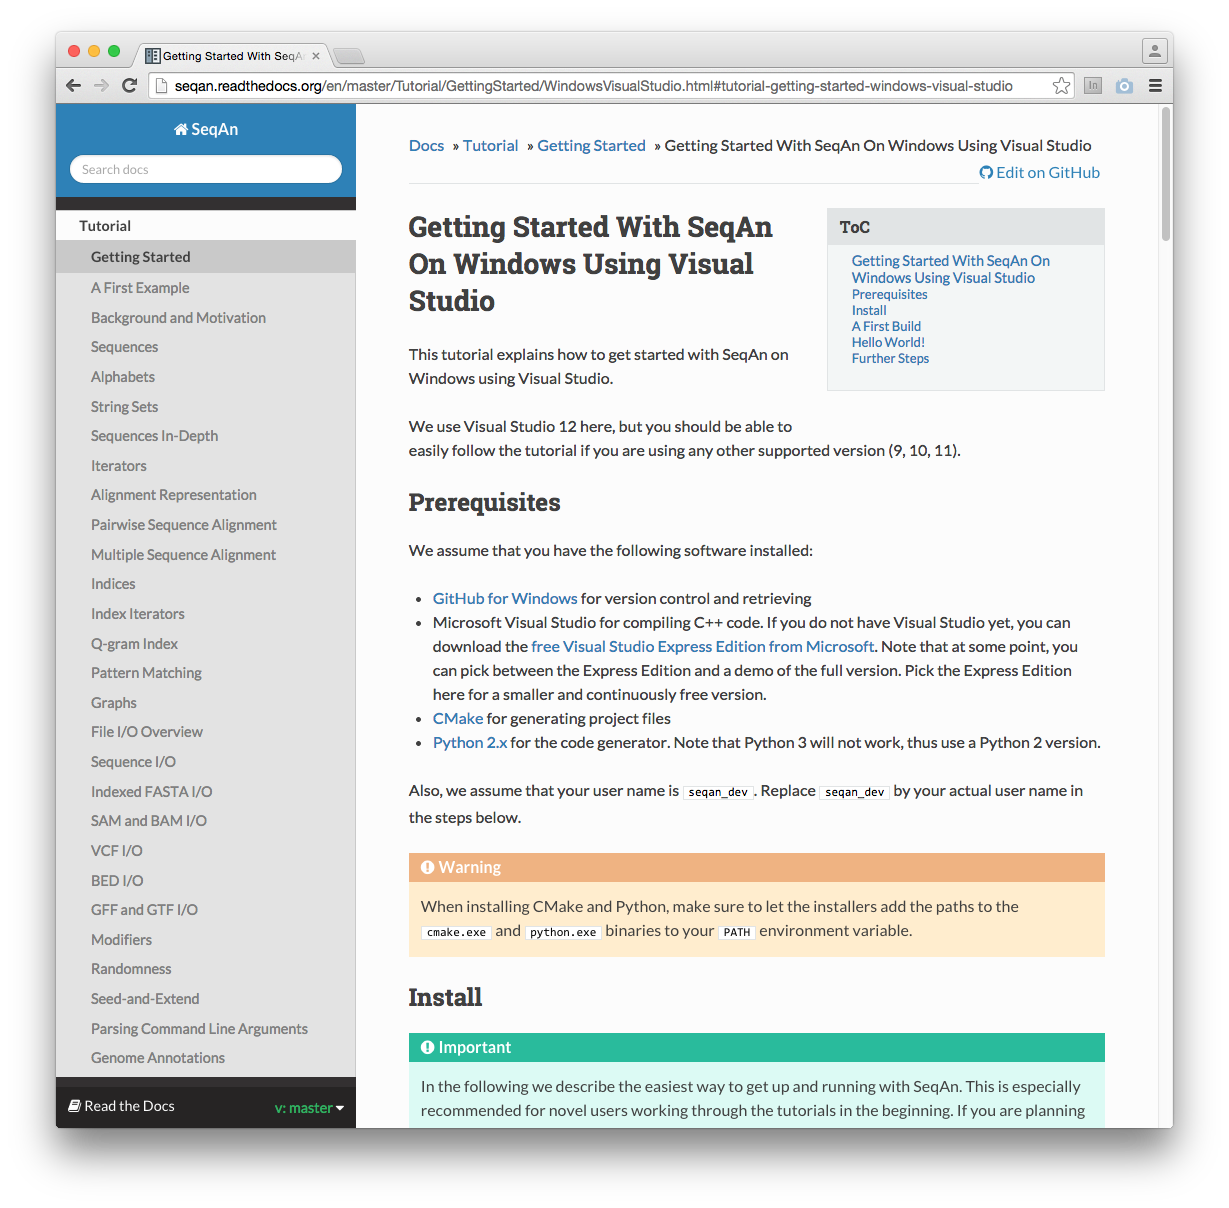
\includegraphics[width=1.0\linewidth]{Figures/getting-started-windows.png}
  \caption[SeqAn-Installation unter Windows]{Ausschnitt aus der verbesserten SeqAn-Installationsanleitung für Windows}
  \label{fig:getting-started-windows}
\end{figure}



\subsubsection{Dokumentation}

Die Dokumentation wurde über mehrere Iterationen hinweg verbessert. In die Verbesserung flossen neben den hier besprochenen Ergebnissen, insbesondere die im \sref{sec:gt} vorgestellten Ergebnisse der \gls{gtm}-Analyse. Daher wird die überarbeitete Dokumentation ausführlich im \sref{sec:improve-dox} vorgestellt.

Die Abbildungen \ref{fig:dox-index-compare-old} und \ref{fig:dox-index-compare-new} geben einen Eindruck über den Grad der Verbesserung.

\begin{figure}
        \centering
        \begin{subfigure}{0.48\linewidth}
                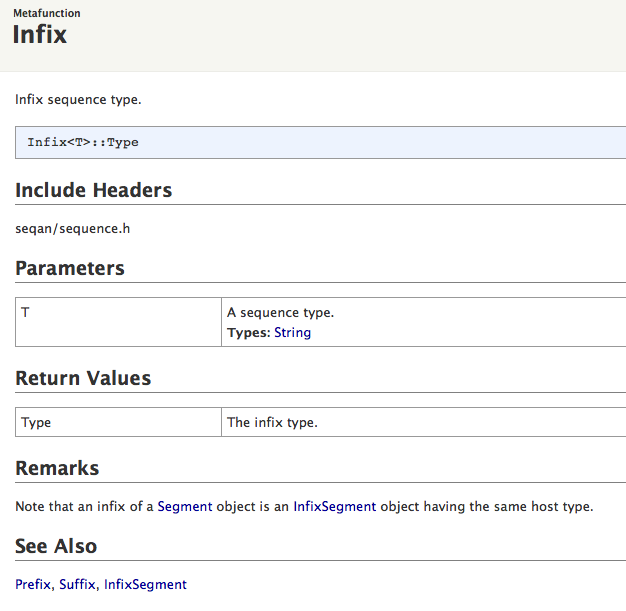
\includegraphics[width=\linewidth]{Figures/dox/infix-old.png}
                  \caption[Vergleich Dokumentationseintrag \texttt{Infix} - Alt]{Alt, Stand: 02.07.2012}
                \label{fig:dox-index-compare-old}
        \end{subfigure}%
        \hfill%
        \begin{subfigure}{0.48\linewidth}%
                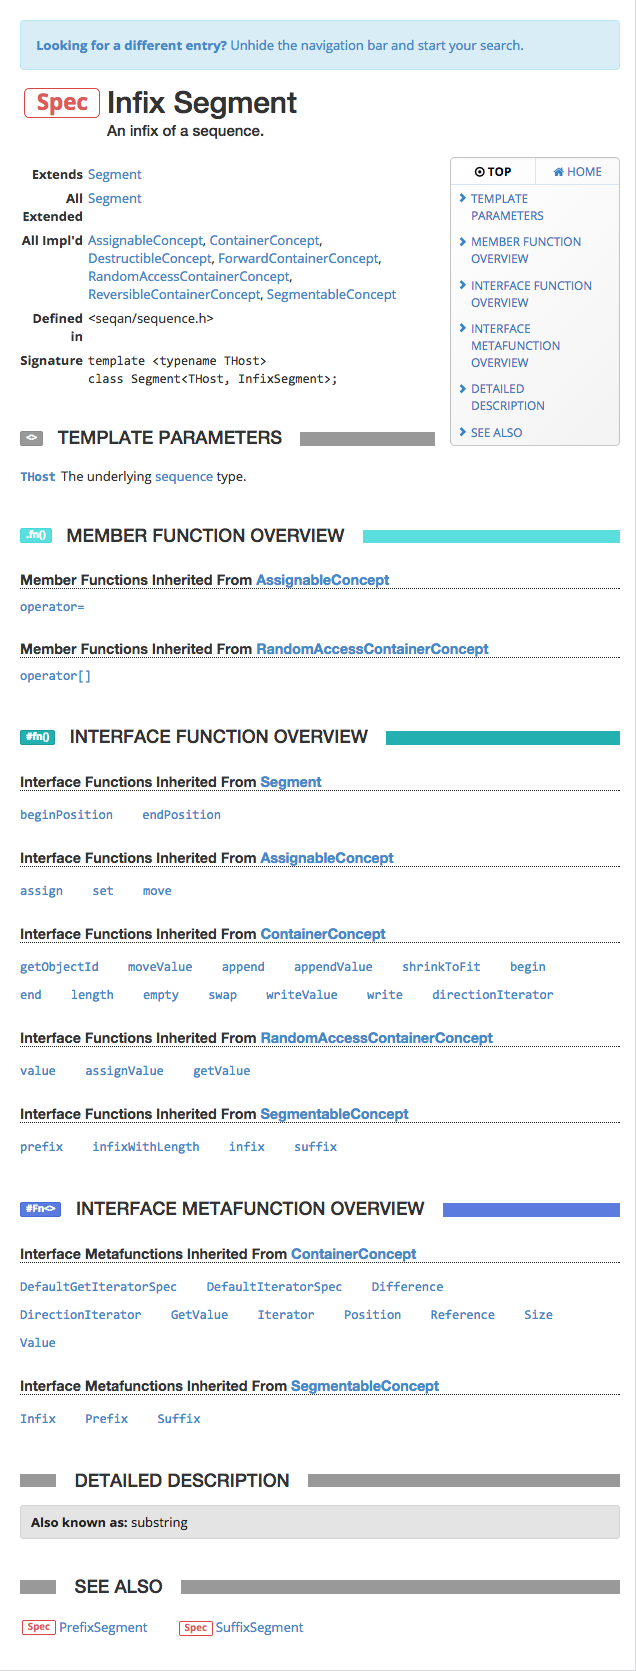
\includegraphics[width=\linewidth]{Figures/dox/infix-new.png}
                \caption[Vergleich Dokumentationseintrag \texttt{Infix} - Neu]{Neu, Stand: 10.04.2015}
                \label{fig:dox-index-compare-new}
        \end{subfigure}%
        \caption{Vergleich Dokumentationseintrag \texttt{Infix}}%
\end{figure}



\subsubsection{Tutorials}
\label{sec:tutorials-improve}

Basierend auf einem etablierten \citep[u.a.][]{Reardon:2008wl,aggarwal2009essentials} Lernphasenmodell \citep{Gagne:1985tx}, den Analyseergebnissen der OOBE-Ressourcen, der Workshops '11 und '12, der PMSB'12-Veranstaltung und einem intensiven Gespräch mit meinen Kollegen am 05.07.2012 --- also knapp ein Jahr nach Beginn der Arbeit --- habe ich die Struktur der Tutorials überarbeitet und Qualitätskriterien formuliert.

Das Ergebnis habe ich in dem Dokument ``Writing Tutorials''\footnote{\url{http://seqan.readthedocs.org/en/master/HowTo/WriteTutorials.html}} zusammengefasst. Es richtet sich an die Autoren von SeqAn-Tutorials und umfasst alle notwendigen Informationen zum Verfassen eines qualitativen Tutorials.

Das eben genannte Dokument ``Writing Tutorials'' verfügt über die folgende Struktur:
\begin{description}
  \item[1. Konventionen] \hfill \\
  Dieser Abschnitt beschreibt, innerhalb eines Tutorials, einzuhaltende Vorgaben.
  \begin{enumerate}
    \item Wiki-Konventionen\\Anforderungen an Wiki-Syntax
    \item Namens-Konventionen\\Anforderungen an Groß- und Kleinschreibung, Benennung des Tutorials, etc.
    \item Design- und Layout-Konventionen\\Anforderung an die Hervorhebung von Schlüsselkonzepten, Verweisen, Programmeingaben und -ausgaben, etc.
  \end{enumerate}
  
  \item[2. Struktur] \hfill \\
  Die Struktur sieht vor, dass ein Tutorial aus einem Meta-Informationen-Block, einer Einführung, inhaltlichen Abschnitten und weiterführenden Links besteht.
  \begin{enumerate}
    \item Meta-Informationen\\Angabe von Lernziel, Schwierigkeitsgrad, voraussichtliche Bearbeitungsdauer und Voraussetzungen mit entsprechenden Links
    \item Einführung\\Tutorial-Inhalt, Relevanz/Wichtigkeit, praktische Anwendungsgebiete und erworbenes Wissen nach Tutorial-Bearbeitung
    \item Abschnitte\\Jeder inhaltliche Abschnitt bespricht einen logischen Lernschritt bestehend aus einem schriftlichen Ausführungen, Beispielen und einer Übungsaufgabe.
    \begin{enumerate}
      \item Einführung\\Abschnittsinhalt, Nennung wichtiger Konzepte, Lernziel
      \item Erklärung\\Eigentlicher Inhalt
      \item Beispiele\\Beispiele, die die Erklärung veranschaulichen und die Umsetzung in SeqAn demonstrieren
      \item Übungsaufgaben\\Wiederholung bzw. Anwendung des erworbenen Wissens
    \end{enumerate}
  \end{enumerate}
  
  \item[3. Didaktik] \hfill \\
  Dieser Abschnitt soll die Autoren von Tutorials für eine benutzerfreundliche, anwender-zentrische Schreibweise sensibilisieren und motivieren.
  \begin{enumerate}
    \item Übungsaufgaben-Typ\\Erklärung der verschiedenen Typen von Übungsaufgaben 
    \item Zeitbedarf\\Schätzung des Zeitbedarfs von Tutorials und Aufgaben
    \item Sprache\\Gebrauch einer einfachen verständlichen Sprache
    \item Mentales Modell\\Einnahme der Leserperspektive
  \end{enumerate}
  
  \item[4. Integration] \hfill \\
  Dieser Abschnitt erläutert technische Fragestellungen wie Orte, an denen ein Tutorial verlinkt werden muss.
  \item[5. Vorlage] \hfill \\
  Dieser Abschnitt stellt eine Vorlage bereit, die über erklärende und zu ersetzende Platzhalter verfügt. So soll sichergestellt werden, dass die Grundstruktur aller neuen Tutorials konsistent bleibt und den qualitativen Anforderungen genügt.
\end{description}

Während manche Tutorials sehr kurz waren, waren andere außerordentlich ausschweifend formuliert. Bei der Bearbeitung Letzterer, gingen wichtige Informationen und Schlüsselkonzepte in der Masse unter. Aus diesem Grund wurden Elemente eingeführt, die explizit den Typ einer Information grafisch mittels einer farbigen Box hervorheben. Es existieren Boxen für wichtige (orange) und optionale (blau) Inhalte (siehe Abbildungen \ref{fig:tutorial-box-important} und \ref{fig:tutorial-box-info}). Darüber hinaus existieren Boxen für Beispiele (grau), Code-Ausschnitte (ebenfalls grau), Programmausgaben (schwarz) und Übungsaufgaben (beige). Außerdem wurden Schlüsselkonzepte fett hervorgehoben und sämtliche genannten Entitäten, wie Funktionen, mit den entsprechenden Dokumentationseinträgen verlinkt.

Die Übungsaufgaben waren vor der Verbesserung von unterschiedlicher Qualität und verfügten über didaktische Schwächen. Diese Probleme sollten u.a. durch die enge Kopplung an einen inhaltlichen Abschnitt gelöst werden. Wichtiger jedoch ist, dass Übungsaufgaben nun von einer der drei folgenden Typen sein müssen: \textit{Review}, \textit{Application}, \textit{Transfer}.

\textit{Review}-Übungen beschränken sich auf die reine Wiederholung von Inhalten und sollen lediglich die Verwendung von SeqAn üben. \textit{Application}-Übungen umfassen Aufgaben, bei denen Variationen vorgenommen werden müssen (z.B. Belegung eines optionalen Parameters). \textit{Transfer}-Übungen sind die anspruchsvollsten und sollen verschiedene Anwendungsmöglichkeiten für das erworbene Wissen aufzeigen.

Eine Forderung an die Übungen ist, dass sie nur in aufsteigender Schwierigkeitsreihenfolge auftauchen dürfen und sich aufeinander beziehen müssen. Beispielsweise darf keine \textit{Review}-Übung auf eine \textit{Application}-Übung folgen. \textbf{Gäbe es tatsächlich für solch einen Fall einen Bedarf, ist das Tutorial wahrscheinlich zu umfassend und muss aufgetrennt werden.} 

\begin{figure}
        \centering
        \begin{subfigure}{0.48\linewidth}
                \raisebox{1.1cm}{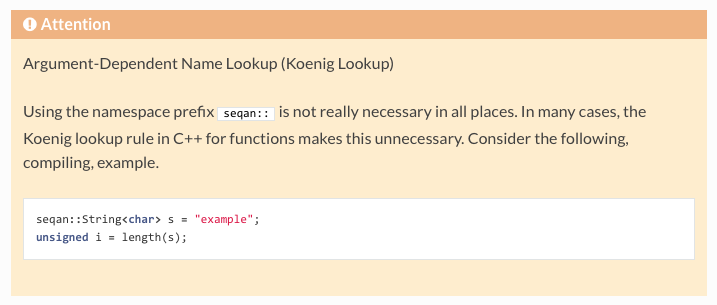
\includegraphics[width=\linewidth]{Figures/tutorial-box-important.png}}
                  \caption{Box für wichtige Inhalte}
                \label{fig:tutorial-box-important}
        \end{subfigure}%
        \hfill%
        \begin{subfigure}{0.48\linewidth}%
                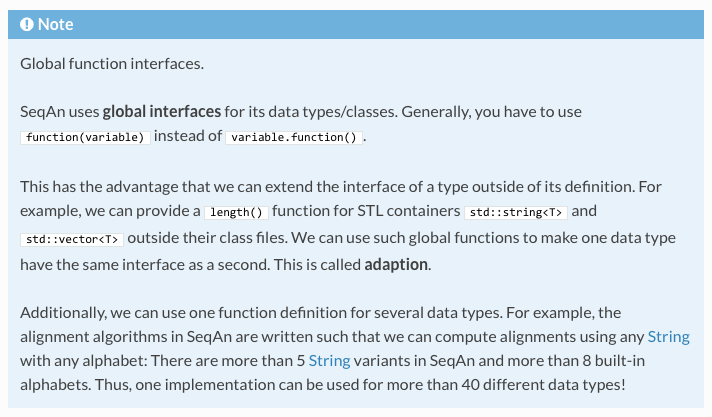
\includegraphics[width=\linewidth]{Figures/tutorial-box-info.png}
                \caption{Box für weiterführende Inhalte}
                \label{fig:tutorial-box-info}
        \end{subfigure}%
        \caption{Boxen zur Auszeichnung von Inhaltstypen}%
\end{figure}

Es wurden mehrere neue Tutorials durch das Auftrennen existierender Tutorials verfasst. Besonders erwähnenswert ist dabei das neue Anfänger-Tutorial ``A First Example''\footnote{\url{http://seqan.readthedocs.org/en/master/Tutorial/FirstStepsInSeqAn.html}}, das eine besonders geringe Einstiegshürde aufweist. Dazu führt es in einfachste Konzepte von SeqAn ein und wird der Beobachtung gerecht, dass viele Anwender einen OOP-Hintergrund haben. 

Die Tutorials wurden sukzessive über eine längere Diskussionsphase hinweg gemeinsam von mir und den jeweiligen Autoren verbessert  (siehe Abbildungen \ref{fig:tutorial-improved}, \ref{fig:tutorial-revisioned} und \ref{fig:tutorial-improved2}). Zum Workshop'12 waren die wichtigsten und zum Workshop'13 alle Tutorials überarbeitet.

\begin{figure}
  \centering
    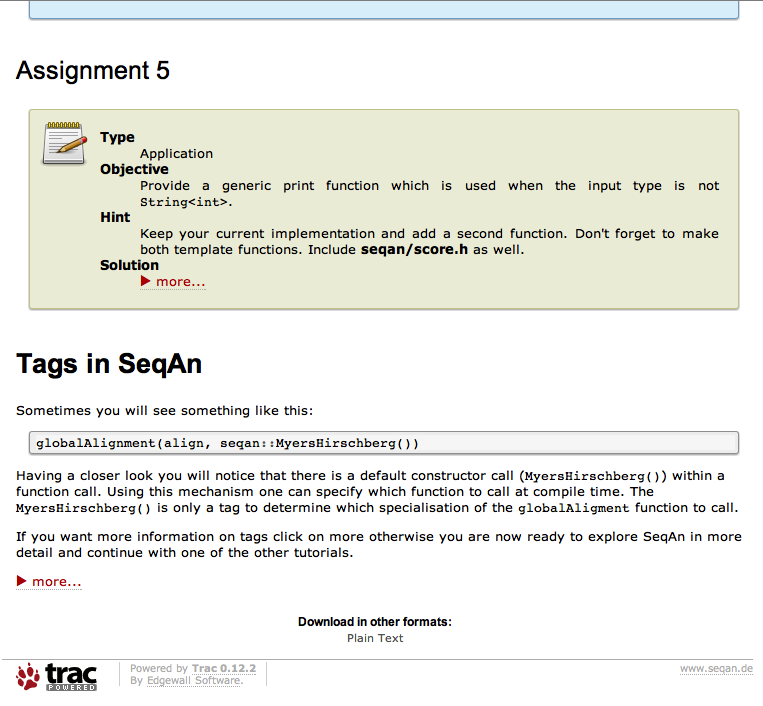
\includegraphics[width=0.57\linewidth]{Figures/tutorial-improved.png}
  \caption{Erste Verbesserung des neuen Anfänger-Tutorials}
  \label{fig:tutorial-improved}
\end{figure}

\begin{figure}
  \centering
    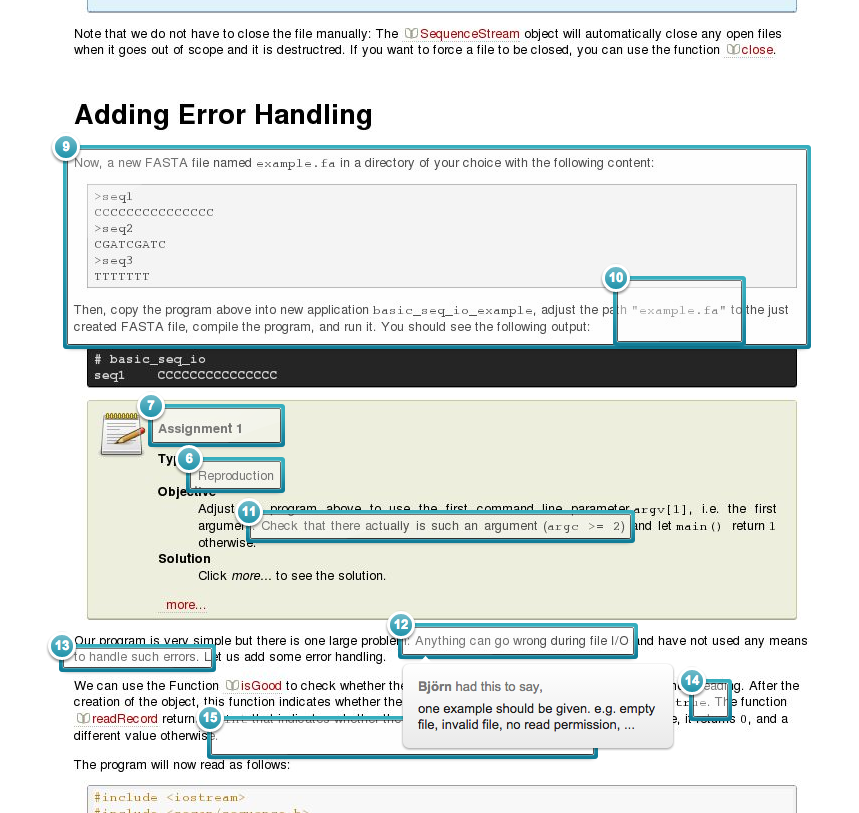
\includegraphics[width=0.65\linewidth]{Figures/tutorial-revisioned.png}
  \caption{Revision der ersten Verbesserung des neuen Anfänger-Tutorials}
  \label{fig:tutorial-revisioned}
\end{figure}

\begin{figure}
  \centering
    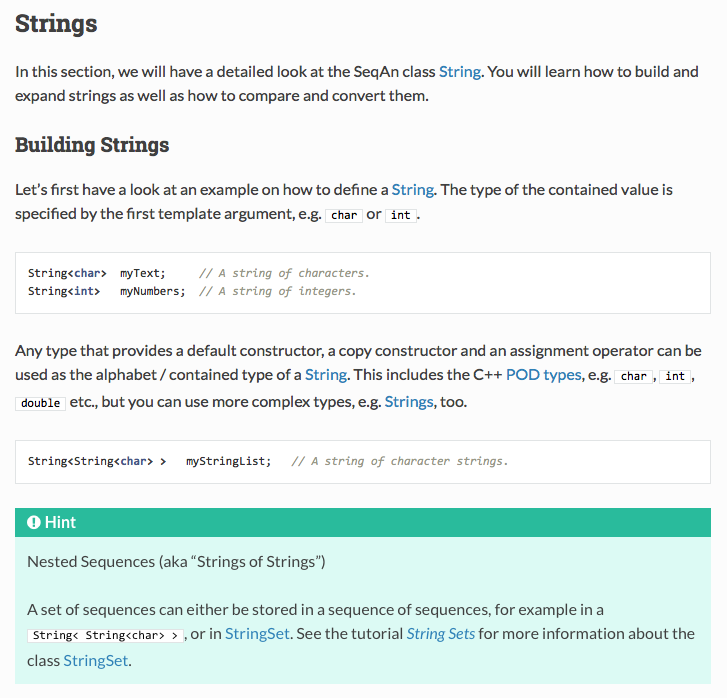
\includegraphics[width=0.55\linewidth]{Figures/tutorial-improved2.png}
  \caption{Zweite Verbesserung des neuen Anfänger-Tutorials}
  \label{fig:tutorial-improved2}
\end{figure}




\subsection{Validierung}
\label{sec:phase1-validierung}

In diesem Abschnitt bespreche ich, wie ich die eben vorgestellten Verbesserungen validiert habe.

\subsubsection{Prozessverbesserungen}

\paragraph{Commit-Nachrichten} Die Vorstellung des neuen Commit-Nachrichtenformats wurde während einer Vorstellung vom SeqAn-Team positiv angenommen. Fast alle darauffolgenden Commit-Nachrichten hielten sich an das Format und vielen deutlicher genauer aus. Als Beispiel habe ich zwei Commit-Nachrichten ausgewählt und jeweils eine inhaltlich passende spätere Commit-Nachricht ermittelt.

\begin{description}
  \item[Beispiel 1] \hfill
  \begin{description}
    \item[Vorher] ``RazerS3: Fixing mate pair modus, deferred compaction.''
    \item[Nachher] ``[FIX] Always adding option -{}-thread-count for RazerS 3, but hiding it in sequential mode.''
  \end{description}
  
  \item[Beispiel 2] \hfill
  \begin{description}
    \item[Vorher] ``Disabling parallel STL in fiona on MinGW.''
    \item[Nachher] ``[API] removed assertions from arg\_parse value accession methods, changed behavior of getValue methods\\
- previously, an assertion ensured that no unset value was requested from the ArgumentParser\\
- now, the method will just not alter the passed reference or will return empty values respectively''
  \end{description}
\end{description}

\paragraph{Umstellung Subversion auf Git}

Die Umstellung auf Git wurde mit dem SeqAn-Team besprochen und eine Einführung wurde gegeben. Alle SeqAn-Entwickler arbeiten zentral und lokal mit Git und können nun lokale Revisionen erstellen, ohne das zentrale Repository zu kompromittieren. Zuvor kam es immer wieder zu Commits, die das Bauen von SeqAn verhinderte.

\paragraph{Code-Reviews}

Die Code-Reviews wurden gut angenommen. Im späteren Verlauf wurde das Prä-Commit-Verfahren auf ein Post-Commit-Verfahren umgestellt. Für Externe gilt weiterhin das Prä-Commit-Verfahren. Ich habe die Codequalität von SeqAn nicht weiter verfolgt, weil ich dieser Verbesserung in Anbetracht meiner eigentlichen \gls{gtm}-Forschung keinen weiteren Raum einräumen wollte. Die gute Annahme seitens der SeqAn-Entwickler deutet aber darauf hin, dass sich die Code-Qualität verbessert hat.


\subsubsection{Argument-Parser}

Sämtliche SeqAn-Anwendungen wurden auf den neuen Argument-Parser umgestellt. Bei der Vorstellung dieses Parsers auf den folgenden Workshops gab es durchweg positives Feedback. Ein Workshop-Teilnehmer sah darin sogar einen Grund, SeqAn allein aus diesem Grund zu verwenden.


\subsubsection{Installation}

Die Installationsanleitungen wurden vollständig überarbeiteten und angeglichenen. Konkrete Hürden bei der Installation von SeqAn (insbesondere unter Windows), wurden auf technischer Seite beseitigt.

Während der Workshops gab es durchweg positives Feedback. Ein Anwender war über die Befragung zu den Installationsanleitungen sogar überrascht und bezeichnete sie als ``vollkommen problemlos''. Ein PMSB'13-Teilnehmer beurteilte die Installationsanleitung als ``idiotensicher''.

Vor der Verbesserung bewertete die Hälfte der Workshop-Teilnehmer die Installation als ``einfach'' oder ``sehr einfach''. Nach der Verbesserung waren es 85\%. Unter den Windows- und Mac-Anwendern kam es zu der deutlichsten Verbesserung.


\subsubsection{Dokumentation}

Die Verbesserung der Dokumentation wird im \sref{sec:improve-dox} und die dazugehörige Validierung im \sref{sec:validierung} besprochen.



\subsubsection{Tutorials}

Die Tutorials sind neben der Dokumentation die wichtigsten Lernressourcen für SeqAn-Anwender. Daher habe ich die Validierung sowohl argumentativ, als auch empirisch vorgenommen. 

\paragraph{Argumentative Validierung}

Bei der Aufgabe des Lernens werden acht sequentielle Phasen durchlaufen \citep{Gagne:1985tx,aggarwal2009essentials}. \cite{Reardon:2008wl} formuliert Instruktionen, die diese Phasen unterstützen und in den SeqAn-Tutorials wie folgt umgesetzt wurden: 

\begin{description}
  \item[1. Motivationsphase] \hfill \\
  Diese Phase wird durch die Tutorial-Metainformationen und -Einführung bedient. Der Anwender kann auf der Grundlage dieser Informationen entscheiden, ob und in welchem Umfang ihn das Tutorial helfen kann. Das gleiche trifft auf die Einführungen der inhaltlichen Abschnitte zu.
  \item[2. Wahrnehmungsphase] \hfill \\
  Durch den Einsatz von typisierten Informationen (z.B. blaue Box für optionale Inhalte) werden wesentliche, von wichtigen und weiterführenden Informationen unterschieden. Durch die unterschiedliche visuelle Darstellung, kann der Anwender schnell diese Informationstypen wahrnehmen.
  \item[3. Akquisitionsphase] \hfill \\
  Diese Phase wird durch Beispiele und Übungsaufgaben des Typs \textit{Review} unterstützt, indem eben wahrgenommenes Wissen verfestigt wird.
  \item[4. Retentionsphase] \hfill \\
  Diese Phase beschreibt die Speicherung von Informationen im Gehirn des Lernenden und kann nicht beeinflusst werden.
  \item[5. Abrufphase] \hfill \\
  Diese Phase wird durch Übungsaufgaben des Typs \textit{Application} unterstützt, indem gespeichertes Wissen, erneut abgerufen und damit verfestigt wird.
  \item[6. Generalisierungsphase] \hfill \\
  Diese Phase wird durch Beispiele und Übungsaufgaben des Typs \textit{Transfer} unterstützt, indem gespeichertes Wissen auf verwandte Aufgabenstellungen angewendet werden muss.
  \item[7. Durchführungsphase] \hfill \\
  Diese Phase wird geringfügig durch die Angabe der voraussichtlichen Bearbeitungsdauer einer jeden Übungsaufgabe unterstützt.
  \item[8. Rückmeldungsphase] \hfill \\
  Diese Phase wird durch die Bereitstellung vollständiger und kompilierbarer Teil- und Gesamtlösungen zu den Übungsaufgaben unterstützt.
\end{description}

Darüber hinaus wird der Anwender durch die Angabe weiterführender Tutorials inspiriert und über weitere Anwendungsgebiete von SeqAn informiert.


\paragraph{Empirische Validierung}

Das neue Einführungs-Tutorial ``A First Example'' wurde sehr positiv von den Workshop'12- und PMSB'12-Teilnehmern angenommen.  80\% der Befragten bewerten dieses Tutorial als überdurchschnittlich (40\%) bzw. außergewöhnlich hilfreich (40\%).

Wurden die Tutorials in ihrer Gesamtheit während des Workshops'11 nur von 24\% als gut oder besser bewertet, waren das nach der Verbesserung zum Workshop'12 ganze 67\%.

Bei der PMSB'12-Befragung gab es durchweg sehr gute Bewertungen, die aber durch die enge Zusammenarbeit mit den SeqAn-Entwicklern verzerrt sein könnte und damit nicht für die Validierung verwendet werden können.